\chapter{Mathematical foundations}
\section{Probability theory}
Homomorphic encryption schemes are based on noise. As we will see in Subsection \ref{subsec:LWE}, noise can be sampled from discrete spaces in accordance with a distribution. Since distributions are central in cryptography, it is important they are understood. A distribution is a probability measure on a measurable space $(S, \mathcal{S})$. Typically, probability distributions are associated with random variables; however, in the absence of random variables, distributions are understood as a specified measure function on the given measurable space (See \cite[pp. 83]{kallenberg-probability}).
\begin{definition}[Discrete distribution measure of a random variable]
Consider a probability space $(\Omega, \mathcal{F}, \operatorname{Pr})$ and a discrete measurable space $(S,\mathcal{S})$. Let $X \colon \Omega \mapsto S$ be a random variable. The discrete distribution measure of $X$, or simply \emph{distribution} of $X$, $\chi$ is defined as follows
\begin{equation*}
\begin{aligned}
    \chi \colon \mathcal{S} &\to [0,1]\\
    \{x\} &\mapsto \operatorname{Pr}[X = x]
\end{aligned}
\end{equation*}
We say that $\chi$ is the distribution or \emph{law} of $X$, denoted $\mathcal{L}(X)$. 
\end{definition}
\begin{remark}
    Since $\chi$ is a measure on a discrete space, the description of the singletons are sufficient. More explicitly, $\chi(A) = \sum_{x \in A} \operatorname{Pr}[X = x]$ for $A \in \mathcal{S}$
\end{remark}
A distribution measure for a random variable is a probability measure on the sample space $(S,\mathcal{S})$, as opposed to on the outcome space $(\Omega, \mathcal{F})$. For a given probability space, any random variable $X$ defined on it has a distribution associated with it. We write $x \leftarrow X$ or $x \leftarrow \chi$ for sampling the outcome $x$ from $X$ assuming $\chi$ is its distribution. When $X$ is a space we mean that $x$ is uniformly sampled from $X$.

\begin{definition}[Ensembles] \label{def:prob-ensemble}
    Let $I$ be a countable index set. A \emph{probability ensemble} indexed by $I$ (or just ensemble) is a sequence of random variables $(X_i)_{i \in I}$. A \emph{distribution ensemble} indexed by $I$ is a sequence of distributions $(\chi_i)_{i \in I}$
\end{definition}
In this paper we will exclusively use $\mathbb{N}$ as the index set.
For example, the encryption function is a random variable (PPT algorithm), meaning that a single message $m$ corresponds to many valid ciphertexts. By varying the security parameter of the scheme we construct the probability ensemble $\{Enc(pk,m)\}_{pk \in \mathbb{N}}$
\begin{definition}[Statistical distance] \label{def:statistical-distance}
    Let $S_n$ be finite set for all $n \in \mathbb{N}$ and let $X = (X_n \colon \Omega_n \to S_n)_{n \in \mathbb{N}}$, $Y = (Y_n \colon \Omega_n \to S_n)_{n \in \mathbb{N}}$ be two ensembles. The \emph{statistical distance} is defined as
    \begin{equation*}
        \Delta_{X,Y}(n) \stackrel{\mathrm{def}}{=} \frac{1}{2} \sum_{\alpha \in S_n} |\operatorname{Pr}[X_n = \alpha] - \operatorname{Pr}[Y_n = \alpha]|.
    \end{equation*}
    Let $\chi = \{\chi_n\}_{n \in \mathbb{N}}$, $\psi = \{\psi_n\}_{n \in \mathbb{N}}$ be two discrete distribution ensembles on the same measurable spaces $\{(S_n, \mathcal{S}_n)\}_{n \in \mathbb{N}}$. The statistical distance is defined as
    \begin{equation*}
    \begin{aligned}
        \Delta_{\chi, \psi}(n) \stackrel{\mathrm{def}}{=} \frac{1}{2} \sum_{\alpha \in S_n} |\chi_n(\{\alpha\}) - \psi_n(\{\alpha\})|
    \end{aligned}
    \end{equation*}
\end{definition}
\begin{remark}
    This definition for distribution ensembles assumes every singleton is measurable. A more general definition is $\Delta(\chi, \psi) \stackrel{\mathrm{def}}{=} \sup _{A \in \mathcal{S}}|\chi(A)-\psi(A)|$ 
\end{remark}

\begin{definition}[Negligible function]
    Let $f \colon \mathbb{N} \to [0,1]$. $f$ is negligible if for all positive polynomials $p(\cdot)$, there exists an $N$ such that for all $n>N$, $f(n) < \frac{1}{p(n)}$. We say $f = \operatorname{negl}(n)$.
\end{definition}
\begin{definition}[Perfectly indistinguishable] \label{def:perfectly-indistinguishable}
    Two ensembles (probability or distribution) $X$ and $Y$ are \emph{perfectly indistinguishable} if $\Delta_{X,Y}(n) = 0$ for all $n$.
\end{definition}
\begin{definition}[Statistically indistinguishable] \label{def:statistically-indistinguishable}
    Two ensembles (probability or distribution) $X$ and $Y$ are \emph{statistically indistinguishable} if $\Delta_{X,Y}(n) = \operatorname{negl}(n)$.
\end{definition}
 A desirable property of encryption schemes is to make it unfeasible for adversaries to distinguish encryptions. For two random variables (or distributions) $X$ and $Y$, we want every adversary $C$ to not be able to distinguish samples from $X$ and $Y$. More precisely, an adversary tasked with identifying whether given samples are from $X$ ($C$ outputs 0) or from $Y$ ($C$ outputs 1) should have roughly the same probability of success irrespective of which the samples are generated from. The formal definition is as follows:
\begin{definition}[Computationally indistinguishable \cite{Gol01}] \label{def:computationally-indistinguishable}
    Two ensembles (or distribution ensembles) $X$ and $Y$ are computationally indistinguishable if, for every polynomial-size circuit family $C = \{C_n\}_{n \in \mathbb{N}}$, $$\operatorname{Adv}_{X,Y}(n) \stackrel{\mathrm{def}}{=} |\operatorname{Pr}[C(X_n) = 1] - \operatorname{Pr}[C(Y_n) = 1]| = \operatorname{negl}(n).$$
\end{definition}
$C(X_n), C(Y_n)$ means that the adversary has access to random oracle returning a sample from $X_n$ and $Y_n$ respectively. The point is that, for every adversary $C$ guessing the samples are from one of the random variables or distributions (1 in this case represents from $Y_n$), the probability of being correct is, up to negligible error, equal to the probability of being incorrect. For example, an adversary always guessing 1 has 100\% probability of being incorrect when given samples from $X_n$ and 100\% probability of being correct when given samples from $Y_n$. The intuition is that the sample does not make a noticable difference on the guess and that the advantage in distinguishing samples goes to zero fast (faster than the inverse of all polynomials).

Perfect distinguishability implies statistical indistinguishability as 0 is negligible. Statistical indistinguishability implies computational indistinguishability. To see why, assume $\Delta_{X,Y}(n) = \operatorname{negl}(n)$ and consider any circuit family $C$. Since $X_n$ and $Y_n$ are defined on the same space we have
\begin{equation*}
\begin{aligned}
    \operatorname{Adv}_{X,Y}(n) &= |\operatorname{Pr}[C(X_n) = 1] - \operatorname{Pr}[C(Y_n) = 1]|\\
        &\leq \sum_{\alpha \in S_n} | \operatorname{Pr}[C(X_n = \alpha) = 1 \; | \; X_n = \alpha]\operatorname{Pr}[X_n = \alpha] \\
        &\phantom{=} \qquad - \operatorname{Pr}[C(Y_n = \alpha) = 1 \; | \; Y_n = \alpha]\operatorname{Pr}[Y_n = \alpha] | \\
        &\leq \sum_{\alpha \in S_n} | \operatorname{Pr}[X_n = \alpha] - \operatorname{Pr}[Y_n = \alpha]| = 2\Delta_{X,Y}(n) = \operatorname{negl}(n)
\end{aligned}
\end{equation*}
where the first inequality is due to the triangle inequality and the second is due to conditional probability being upper bounded by 1. Intuitively, there does not exist enough distinguishable outcomes to distinguish the ensembles even if there exists an adversary that always correctly recognize an outcome from $X$ and $Y$ respectively.
\section{Discrete Gaussian Distribution}
To add discrete noise to ciphertexts, it is typical to use the discretized Gaussian distribution introduced by Micciancio and Regev \cite{disc-gauss}. Since this distribution is used so frequently, we give a brief presentation of it here. A continuous Gaussian distribution in $\mathbb{R}^n$ centered at $\vec{c}$ where each coordinate is independently sampled from normal distirbution with standard deviation $\sigma$, then the multivariate Gaussian distribution is simplified to $\rho_{\vec{c}}(\vec{x}; \sigma)=\frac{1}{\left(2 \pi \sigma^2\right)^{n / 2}} \exp \left(-\frac{1}{2 \sigma^2} \| \vec{x}-\vec{c} \| ^2\right)$. By introducing the scale factor $s \stackrel{\mathrm{def}}{=} \sqrt{2\pi}\sigma$ we get $\rho_{s, \vec{c}}(\vec{x})=\frac{1}{s^n} \exp \left(-\frac{\pi}{s^2} \| \vec{x}-\vec{c} \| ^2\right)$.
The goal is to discretize the gaussian over lattices, see Section \ref{sec:hard_problems}, by restricting the domain to lattice points. For a given lattice $L \subset \mathbb{R}^n$ we define the normalization constant $\rho_{s, \vec{c}}(L) \stackrel{\mathrm{def}}{=} \sum_{\vec{x} \in L} \rho_{s, \vec{c}}(\vec{x})$.
\begin{definition}[Discrete Gaussian distribution]\label{Disc-Gauss}
    Let $L \subset \mathbb{R}^n$ be a lattice. Then the discrete gaussian distribution is defined as
    \begin{equation*}
        \forall \vec{x} \in L \colon \quad \textrm{D}_{L, s, \vec{c}}(\vec{x}) \stackrel{\mathrm{def}}{=} \frac{\rho_{s, \vec{c}}(\vec{x})}{\rho_{s, \vec{c}}(L)}.
    \end{equation*}            
\end{definition}
\begin{definition}[$\beta$-bounded distribution]
    Let $\chi$ be a distribution over the integers. $\chi$ is $\beta$-bounded if $x \leftarrow \chi \implies |x| < \beta$
\end{definition}
\begin{remark}
    It is also possible (and common) to define a $\beta$-bounded distribution such that $|x| \geq \beta$ with negligible probability.
\end{remark}
\begin{figure}
    \centering
    \hypertarget{fig:discrete-gauss}{}
    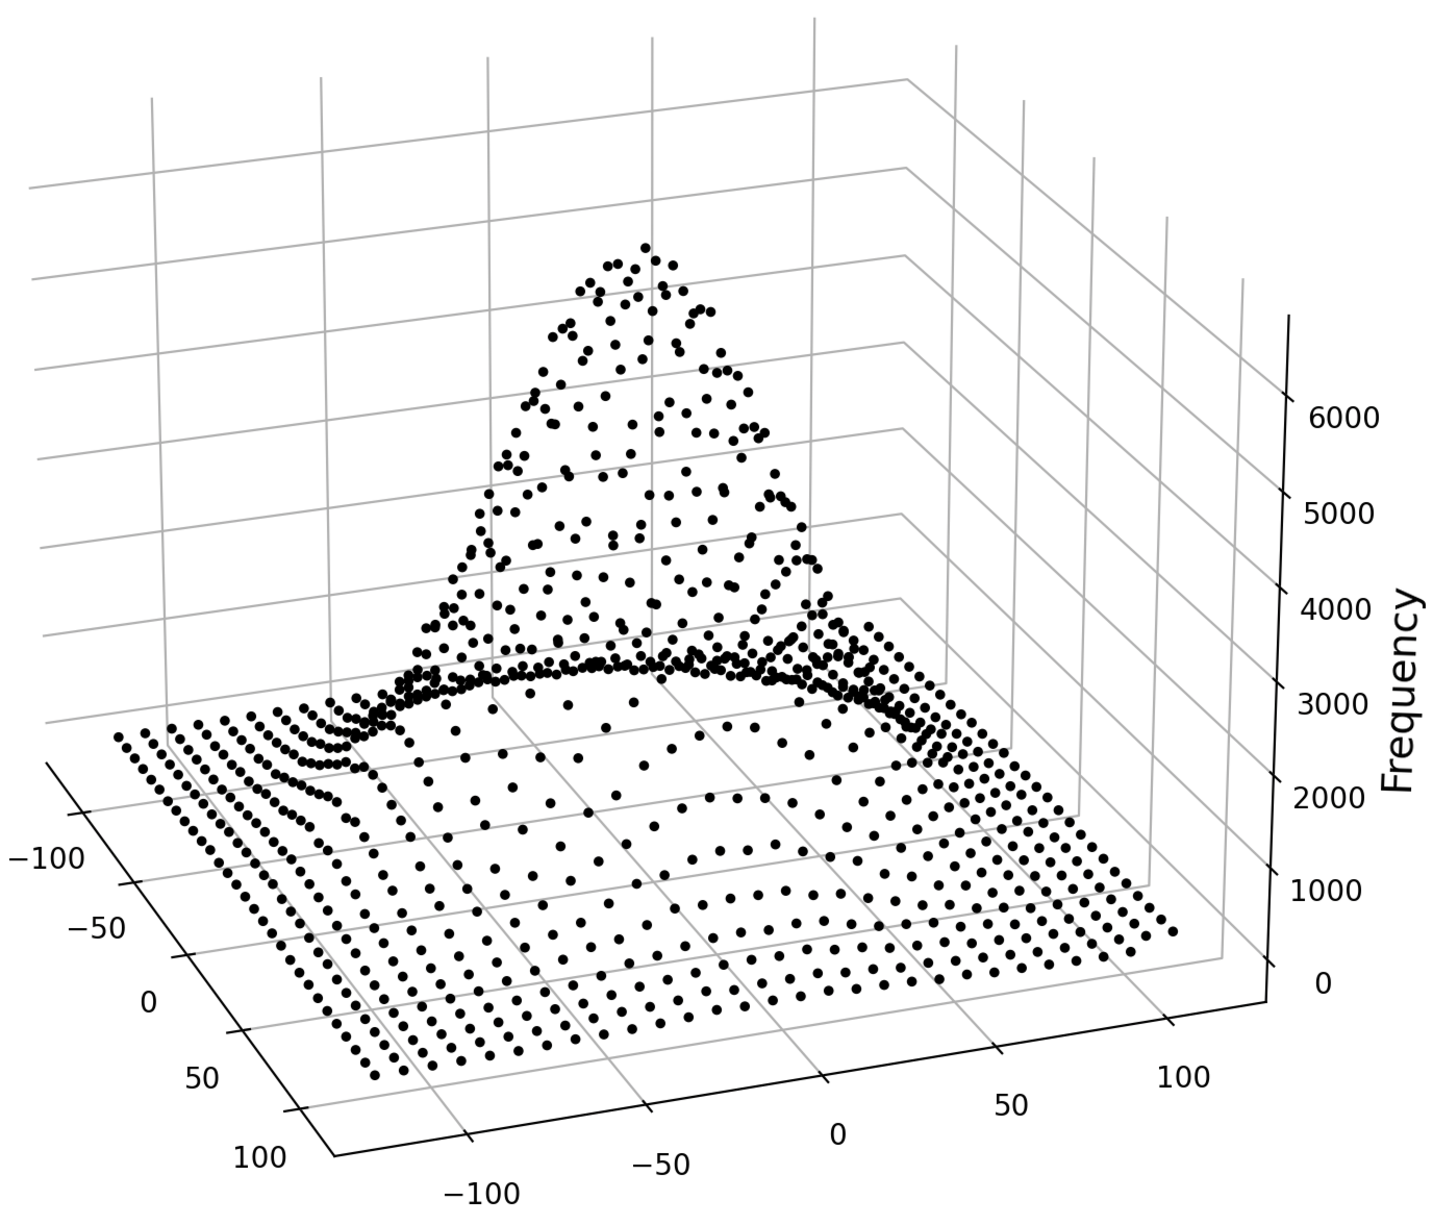
\includegraphics[width=0.65\textwidth]{figures/D-G-2d-a_is_100-n_1000000.pdf}
    \caption*{\textbf{Figure 1}: Discrete Gaussian distribution $\textrm{D}_{\mathbb{Z}^2, 100, \vec{0}}$ with 1 million samples. Every point has integer coordinates. See code in Appendix \ref{app:code}.}
\end{figure}

\subsection*{Subgaussian distributions}
In this section we introduce subgaussian distributions. We use subgaussian distributions for a tighter error analysis when discussing the GSW scheme in Chapter \ref{ch:implementation}. Much of this section can be found in \cite{A-S-P-boot}.
\begin{definition}[Subgaussian distribution]
    A distribution $\chi$ over $\mathbb{R}$ is subgaussian with parameter $K > 0$ ($K$ not nesessarily constant) if for every non negative $t \in \mathbb{R}$.
    \begin{equation*}
        \chi(\{x \in \mathbb{R} \text{ such that} \; |x| > t\}) \leq 2e^{- \pi \frac{t^2}{K^2}}
    \end{equation*}
    Or equivalently, a real valued random variable $X$ has subgaussian distribution if
    \begin{equation*}
        \operatorname{Pr}[|X|>t] \leq 2e^{- \pi \frac{t^2}{K^2}}
    \end{equation*}
    We say $X$ is a subgaussian random variable.
\end{definition}
The intuition of subgaussian distributions is that the probability of a random variable $X$ being taking a large value is less than the probability of a Gaussian taking the same value. In other words, the tails of a subgaussian distribution decays at least as fast as the tails of a Gaussian distribution. In particular, the $\beta$-bounded distributions are subgaussian with parameter $\beta \sqrt{2\pi}$. To see why, clearly, for all $t \geq \beta$, $\operatorname{Pr}[|X|>t] = 0$ whereas the exponential function is non-negative. Furthermore, for $t < \beta$ we have $2e^{- \pi \frac{t^2}{2\pi \beta^2}} > 2e^{- \pi \frac{\beta^2}{2\pi \beta^2}} = 2e^{-\frac{1}{2}} > 1 > \operatorname{Pr}[|X|>t]$. Hence, the definition is satisfied for all non-negative $t$.

Subgaussian variables are closed under scalar multiplication in the sense that if $X$ is a subgaussian random variable with parameter $K$, then for any non-zero real number $a$, $aX$ is subgaussian with parameter $|a|K$. This follows from $\operatorname{Pr}[|aX|>t] = \operatorname{Pr}[|X|>\frac{t}{|a|}] \leq 2e^{- \pi \frac{t^2}{(|a|K)^2}}$. Furthermore, it can be shown by using moment generating functions that a finite sum of $n$ subgaussian random variables with parameters $K_1, \dots, K_n$ is subgaussian with parameter $\sqrt{\sum_{i=1}^n K_i^2}$.

We extend the definition of subgaussian random variables to vectors of subgaussian random variables. Let $u \in \mathbb{R}^n$ be any fixed unit vector and let $\vec{X} = (X_1, \dots, X_n)$ be a vector of random variables. We say $\vec{X}$ is subgaussian with parameter $K$ if $\left\langle u,\vec{X} \right\rangle$ is subgaussian with parameter $K$. The intuition is that for any direction, the probability of sampling points far away from origin decays at least as fast as a gaussian. Our focus is on random vectors of independent subgaussian entries. In this case, the vector is subgaussian with the same parameter as the maximum parameter of the entries (see Proposition 5.10 in \cite{vershynin2011introduction}). In other words, let $\vec{X} = (X_1, \dots, X_n)$ be a vector of independent subgaussian random variables with parameters $K_1, \dots, K_n$. Then $\vec{X}$ is subgaussian with parameter $\underset{i \in [n]}{\max} \ K_i$.

By considering each element individually, it is clear that multiplication with non-negative scalar and addition of vectors preserves subgaussianity in the same way. An important application is the inner product of a vector with a subgaussian vector. Let $\vec{e} = (e_1, \dots, e_n)$ be a vector of independent entries where each entry is sampled from a $\beta$-bounded distribution (i.e., $\vec{e}$ is subgaussian). Let $\vec{X} = (X_1, \dots, X_n)$ be a vector of independent subgaussian random variables with parameters $K_1, \dots, K_n$ for some fixed constants $K_1, \dots, K_n$. Denoting $K = \underset{i \in [n]}{\max} \ K_i$ then gives $\left\langle \vec{e}, \vec{X} \right\rangle$ is subgaussian with parameter $\sqrt{\sum_{i=1}^n e_i^2 K_i^2} \leq K \sqrt{\sum_{i=1}^n e_i^2 } = K \| \vec{e} \| = O(\|\vec{e}\|)$. 
As a last point, we introduce a bound on the euclidean norm of a subgaussian vector.
\begin{theorem}[Lemma 2.1 \cite{A-S-P-boot}]
    Let $\vec{X}$ be an $n$ dimensional subgaussian vector with parameter $K$, containing mutually independent entries. Then there exists real positive constant $C$ such that 
    \begin{equation*}
        \operatorname{Pr}[\| \vec{X} \| > CK\sqrt{n}] \leq 2^{-\Omega(n)}
    \end{equation*}
\end{theorem}
In particular, the length $\| \vec{X}\|$ is $O(K\sqrt{n})$ except with negligible probability.

\section{Embedding integers as permutations}
In this section we show how to embed integers in a finite group as a tuple of cyclic shifts by showing $\mathbb{Z}_q \cong S_{r_1} \times \dots \times S_{r_t}$ where $q = \prod_{i=1}^t r_i$ for pairwise coprime $r_i$. Representing integers in this way is nesessary for the error analysis in the implementation of the GSW scheme, see Chapter \ref{ch:implementation}. The isomorphism is established through the Chinese Remainder Theorem and Cayley's theorem.
\begin{theorem}[Chinese Remainder Theorem]
    Let $r_1, \dots, r_t$ be pairwise coprime integers and $q = \prod_{i=1}^t r_i$.
    The system of congruences
    \begin{equation*}
    \begin{array}{rl}
        x & \equiv a_1 \pmod{r_1} \\
        &  \vdots \\
        x & \equiv a_t \pmod{r_t} \\
    \end{array}
    \end{equation*}
    has a unique solution $x \in \mathbb{Z}_q$.
    We say $(a_1, \dots, a_t)$ is the RNS representation of $x$ with respect to the moduli set $\{r_1, \dots, r_t\}$.
\end{theorem}
The Chinese Remainder Theorem allows us to construct an isomorphism from $\mathbb{Z}_q$ to $\mathbb{Z}_{r_1} \times \dots \times \mathbb{Z}_{r_t}$.
\begin{definition}[CRT isomorphism]
    We define the \textit{CRT isomorphism} $\mathbb{Z}_q \rightarrow \mathbb{Z}_{r_1} \times \dots \times \mathbb{Z}_{r_t}$ as a mapping of $x$ to its RNS representation $(a_1, \dots, a_t)$ with respect to the moduli set $\{r_1, \dots, r_t\}$.
\end{definition}
\begin{remark}
    To compute the CRT isomorphism on a given input $x$ we simply compute $x \bmod r_i$ for each $i$ (we will not need the inverse mapping but it can be computed using the Extended Euclidean Algorithm).
\end{remark}
We will now discuss how to embed the finite additive group $\mathbb{Z}_r$ into the symmetric group $S_r$. The symmetric group $S_r$ is the group of all permutations of the set $\{1, \dots, q\}$. A standard way to represent a permutation $\pi \colon \{(x_1, \dots, x_r) \mid x_a \neq x_b, \; a,b \in [r]\} \to \{(x_1, \dots, x_r) \mid x_a \neq x_b, \; a,b \in [r]\}$ in $S_r$ is to list where each entry is mapped to; $(x_1,\dots,x_r) \stackrel{\pi}{\mapsto} (\pi(x_1), \dots, \pi(x_r))$. In this paper we will use a binary representation by using a square permutation matrix $M^{\pi} \in \{0,1\}^{r \times r}$ such that $M^{\pi}_{i, j} = 1$ if and only if $\pi$ maps the $j$:th entry to the $i$:th entry. In other words, column $j$ represents the mapping of element $j$. Since every entry is mapped to exactly one other entry, every column has exactly 1 non-zero entry. Since a permutations is a bijection, surjectivity implies every row has a non-zero entry. Therefore, every row and every column has exactly 1 non-zero element. $M^{\pi}$ contains exactly $r$ entries equal to 1 and $r^2 - r$ entries equal to 0. For example, consider a cyclic shift permutation $\pi \in S_3$ defined as $(\pi(x_1),\pi(x_2),\pi(x_3))=(x_3,x_1,x_2)$. Then the corresponding permutation matrix $M^{\pi}$ is
\begin{equation*}
    M^{\pi} = \begin{pmatrix}
        0 & 0 & 1 \\
        1 & 0 & 0 \\
        0 & 1 & 0
    \end{pmatrix}.
\end{equation*}
A particular permutation group of interest is the cyclic shift group $C_r$. $C_r$ is the subgroup of the symmetric group $S_r$ consisting of permutations shifting the input sequence by a fixed number of positions. Every element of this group can be represented by only the first column of the permutation matrix since the shift of the first element in the sequence must be the same as the shift for every other element. In other words, every element of $C_r$ can be represented by a $r$ dimensional indicator vector $\pi \in \{0,1\}^r$. Our above example of a cyclic shift of 1 position to the right can therefore be represented by the indicator vector $\pi = (0,1,0)^T$.  
\begin{theorem}[Cayley's theorem]
    Every group $G$ is isomorphic to a subgroup of the symmetric group $S_{|G|}$.
\end{theorem}
In particular, the additive group $\mathbb{Z}_r$ is isomorphic to $C_r$ through the following natural embedding isomorphism.
\begin{definition}[Embedding isomorphism]
    We define the \textit{embedding isomorphism} $\mathbb{Z}_r \rightarrow C_r$ as a mapping of $x$ to the indicator vector $(b_0, \dots, b_x, \dots, b_{r-1})$ where $b_i = 1$ if and only if $i = x$.
\end{definition}
By using the CRT isomorphism and the embedding isomorphism we can represent an element in $\mathbb{Z}_q$ as a direct sum of cyclic shifts.
Consider the following example showing how to represent an element in $\mathbb{Z}_q$ into $S_{r_1} \times \dots \times S_{r_t}$.
Say we want to represent the integer $7 \in \mathbb{Z}_{15}$ as a direct sum of cyclic shifts. I.e., $q = 15 = 3 \times 5$, $t = 2$, $r_1 = 3$ and $r_2 = 5$. We have $x \bmod 3 = 1$ and $x \bmod 5 = 2$. The RNS representation of $7$ is therefore $(1,2)$ with respect to the moduli set $\{3,5\}$. We can now represent $x$ in $S_3 \times S_5$ by using the embedding isomorphism on each element of the RNS representation. We have $(1,2) \mapsto ((0,1,0)^T, (0,0,1,0,0)^T)$. Thus, the element $7$ in $\mathbb{Z}_{15}$ is represented by a tuple of two cyclic shifts, $((0,1,0)^T, (0,0,1,0,0)^T) \in S_3 \times S_5$.

\subsection{Efficient representation of integers as cyclic shifts}
As it stands, representing integers as cyclic shifts can be innefficient. For instance, for a prime $q$, an element in $\mathbb{Z}_q$ is represented in binary using $\log q$ bits whereas the corresponding cyclic shift is represented with an indicator vector using $q$ bits, thus yielding an exponential expansion in the representation size. For cyclic shift representation to be efficient, we want to choose modulus $q$ yielding pseudo-constant bit size representation. In other words, the goal is to guarantee choise of $q$ such that representing an integer using a tuple of cyclic shifts requires $O(\operatorname{polylog(q)})$ bits. To do so, we want to find $q = \prod_{i=1}^t r_i$ such that $\underset{i \in [t]}{\max} \ r_i = O(\log q)$ and $t = O(\frac{\log q}{\log \log q})$. This would yield that every $x \in S_{r_1} \times \dots \times S_{r_t}$ can be represented in $O(\frac{\log^2q}{\log \log q}) = \tilde{O}(1)$. We will now show that such a modulus $q$ exists and how to find it.

\begin{definition}
    The maximal prime powers bounded by an positive integer $r$ is defined as the set
    \begin{equation*}
        \text{MPP}(r) \stackrel{\mathrm{def}}{=} \{p^{\lfloor \log_p r \rfloor} | \; p \leq r, \text{ p is prime}\}.
    \end{equation*}
    An element in $\text{MPP}(r)$ is called a maximal prime power.
\end{definition}
For example, the maximal prime powers bounded by $10$ is $\text{MPP}(10) = \{2^3, 3^2, 5^1, 7^1\} = \{8,9,5,7\}$.

\begin{theorem}[Lemma 2.2 \cite{A-S-P-boot}]\label{thm:lemma2.2}
    Let $r \geq 7$ be an integer. Then
    \begin{equation*}
        \underset{r_i \in \text{MPP}(r)}{\prod} r_i \geq e^{\frac{3r}{4}}.
    \end{equation*}
\end{theorem}

The idea is to choose $q$ as the product of maximal prime powers bounded by some $r = O(\log q)$. In other words, we consider $t = |\text{MPP}(r)|$ and $\{r_1, \dots, r_t\} = \text{MPP}(r)$. We can efficiently find such $q$ by first determining an acceptable lower bound $q_0 \leq q$. Since $r \geq 7$, we require $q_0 \geq e^{\frac{3 \times 7}{4}} > 190$. The second step is to find an $r$ such that the product of its maximal prime powers is greater than or equal to our lower bound $q_0$. Choosing $r = \lceil \frac{4}{3} \log q_0 \rceil$ works since $q = \underset{r_i \in \text{MPP}(r)}{\prod} r_i$ is, by Theorem \ref{thm:lemma2.2}, at least $e^{\frac{3r}{4}} = e^{\frac{3}{4} \lceil \frac{4}{3} \log q_0 \rceil} \geq e^{\log q_0} = q_0$.

Note that $r$ is logarithmic with respect to $q$, implying $\underset{i \in [t]}{\max} \ r_i = O(\log q)$.
We now show that $t = O(\frac{\log q}{\log \log q})$.

\begin{theorem}[Prime number theorem]
    Let $f(x)$ be the number of primes less than or equal to the real value $x$. Then
    \begin{equation*}
        \lim_{x \to \infty} \frac{f(x)}{x/\ln(x)} = 1
    \end{equation*}
\end{theorem}
Note that prime number theorem gives that the number of primes bounded by an integer $x$ is $O(x/\log(x))$. In particular, $\text{MPP}(r)$ contains exactly one element per prime bounded by $r$, meaning $t = O(\frac{r}{\log r}) = O(\frac{\log q}{\log \log q})$.

As an example, say we want a modulus $q \geq 1000$. Then $r = \lceil \frac{4}{3} \log 1000 \rceil = 14$. We have $q = \underset{r_i \in \text{MPP}(14)}{\prod} r_i = 2^3 \times 3^2 \times 5^1 \times 7^1 \times 11^1 \times 13^1 = 360360$. We can now represent an element $x \in \mathbb{Z}_{360360}$ as a tuple of cyclic shifts in $S_8 \times S_9 \times S_5 \times S_7 \times S_{11} \times S_{13}$. Note that $t = |\text{MPP}(14)| = 6 = O(\frac{\log q}{\log \log q})$ and $\underset{i \in [t]}{\max} \ r_i = \max\{\text{MPP}(14)\} = 13 = O(\log q)$.